% !TEX root = paper.tex

\label{sec:nsp-face-auth}

This chapter considers the design of a processing pipeline for an energy-constrained camera, the WISPCam~\cite{wispcam}, a battery-free platform which operates entirely on harvested RF energy.
We characterize a continuous vision pipeline using face authentication (FA), a core workload in user-centric continuous mobile vision systems.
In these systems, a camera captures image frames at a continuous frame rate, and an on-node processor performs face recognition on each frame to identify a user.
These applications are common in biometrics and vision-based personal analytics.
In the design of this system, we investigate ways to use perceptual information


The WISPCam-based system captures an image at 1 frame per second (FPS) and transmits it over RF, powered by an internal capacitor with harvested RF energy.
We examine how leveraging progressive filtering hardware can dramatically reduce the power consumption of such a system and enable continuous face authentication at low cost.
We construct our FA pipeline around a neural network (NN) accelerator performing face authentication, as shown in Figure~\ref{fig:face_recog_pipeline_solution}.


\begin{marginfigure}
  \includegraphics[width=.8\textwidth]{nsp-figs/FA_pipeline_base_with_example.pdf}
  \caption{Face authentication with battery-free cameras. }
  \label{fig:face_recog_pipeline_solution}
\end{marginfigure}

The pipeline has one primary block, the NN, and several optional blocks.
Given the WISP's energy constraints, we design the accelerators to be integrated on-chip with the camera sensor to minimize energy, and processed the pixels streaming through the CSI2 camera serial interface.
Co-designing our accelerators with the streaming camera interface helps optimize our design.

We analyze the algorithmic and microarchitectural choices that can improve the efficiency of such a pipeline while minimizing the impact on accuracy.
We first discuss the hardware accelerators required for the camera pipeline, presenting their microarchitectures and the tradeoffs we investigated in each design's algorithm and hardware implementation.
We then evaluate them together on a real-world face authentication workload using real video we collected.
Our evaluation discusses the performance and power improvements, specifically exploring the tradeoffs in power consumption arising from considering the total cost of computation and communication.

\section{Background: Face Detection and Machine Learning Metrics}
\label{sec:backvj}

\subsection{Viola-Jones algorithm for face detection}

The Viola-Jones (VJ) face detection algorithm is a state-of-the-art computer vision algorithm for fast, accurate face detection \cite{vj_journal}. It detects faces by scanning a window of fixed size across the image, looking for features of a face, such as eyes and nose. If enough of these features are found, then the window at a particular location in the image is identified as a face. To account for faces of different sizes in an image, the scanning window is scaled and passed over the scene multiple times. The face detection process at each window is independent of windows at other positions and scale sizes.

The Viola-Jones algorithm is well-known because of its simplicity and efficiency,
and continues to perform well against more complex algorithms \cite{mathias_fd}.
The algorithm's efficiency stems from three factors: (i) simple feature
designs, (ii) use of an efficient encoding and data layout (i.e., integral images) that reduces data accesses, and (iii) the cascade classifier structure.

\paragraph{Rectangular features.} The features used in the VJ algorithm
are a weighted sum of rectangular pixel areas. These features are referred to
as \textit{Haar-like features} because of their similarity to Haar wavelet
functions, which are natural basis functions for encoding differences in average intensities
between different regions \cite{haar_basis}.
VJ uses three rectangular features (more
recent work has extended the set of features, but we focus on the original three).

A two-rectangle feature is defined to be the difference between the sum of the
pixels within two rectangular regions where the two regions have the same size
and shape and are horizontally or vertically adjacent. Three- and four-rectangle
features are constructed in a similar manner. In a given $20\times 20$ window of image
pixels, the exhaustive set of rectangular features is 160,000. For fast
classification, the VJ framework employs the AdaBoost~\cite{adaboost} learning algorithm to choose a
small set of critical features for detecting faces.

\paragraph{Cascade classifier structure.} While feature computation is fast and efficient, an accurate classifier executes a large number of these computations per window. The VJ algorithm reduces the  computation overhead by ruling out ``easy-to-dismiss'' image windows quickly. This is done by constructing small classifiers from weighted combinations of features, and then grouping these classifiers into successively more complex stages in a cascade structure (Figure~\ref{fig:vj-cascade}).

\begin{marginfigure}
  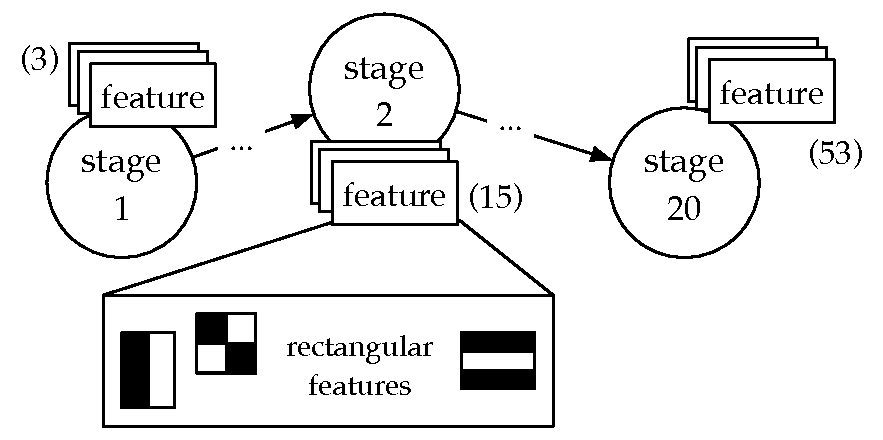
\includegraphics[width=\textwidth]{nsp-figs/cascade_structure.pdf}
  \caption{Features grouped into cascading stages.}
  \label{fig:vj-cascade}
\end{marginfigure}


The first classifier stage searches the image window for a small number of critical features that exist in all the face images. If the window contains all the features, it is processed by the next stage in the sequence of classifiers. Each stage in the sequence is more complex than the last, and if any stage rejects the image window, the classifier stops processing on the window. This cascade classifier structure is similar to a degenerate decision tree.

\paragraph{Integral image.}Computing the rectangular features involves summing across
the pixels in a rectangular area, and taking the average of those pixels.
A data structure called an \emph{integral image} expedites these sum calculations. In this
data structure, the value at any pixel position is the sum of all the pixels value above and
to the left of it.

% \begin{figure}[h]
%      \centering
%      \begin{subfigure}[b]{0.25\textwidth}
%          \centering
%          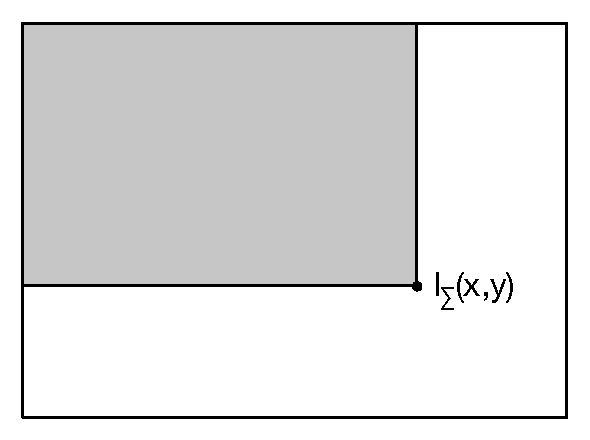
\includegraphics[width=\textwidth]{nsp-figs/integral_image_access.pdf}
%          \caption{Pixels in an integral image are the sum of all the preceding ones.}
%          \label{fig:integral:a}
%      \end{subfigure}
%      \hfill
%      \begin{subfigure}[b]{0.25\textwidth}
%          \centering
%          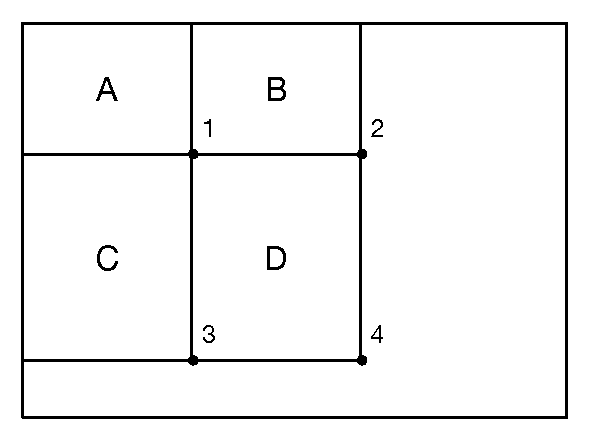
\includegraphics[width=\textwidth]{nsp-figs/integral_feature.pdf}
%          \caption{The rectangular area D can be computed in 4 accesses by the formula: D = 4 + 1 - 2 - 3.}
%          \label{fig:integral:c}
%      \end{subfigure}
%      \hfill
%      \begin{subfigure}[b]{0.25\textwidth}
%          \centering
%          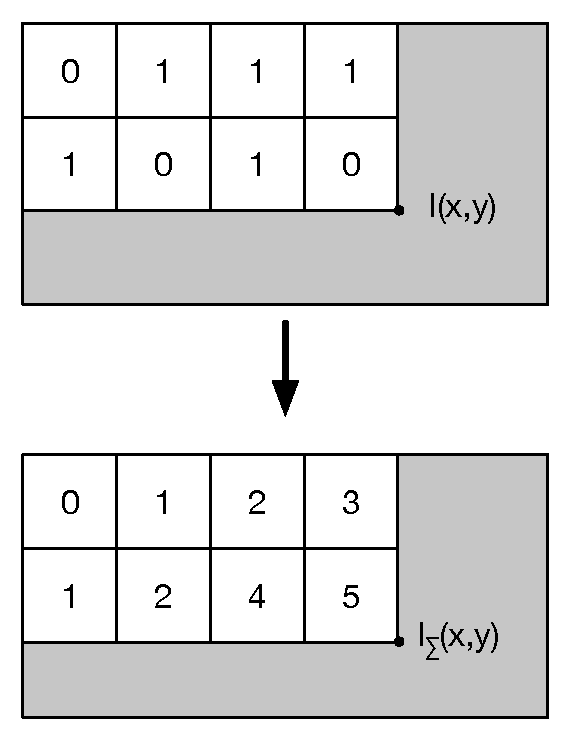
\includegraphics[width=\textwidth]{nsp-figs/integral_image_compute.pdf}
%          \caption{Integral image pixel computation.}
%          \label{fig:integral:b}
%      \end{subfigure}
%         \caption{Computing an integral image.}
%         \label{fig:integral}
% \end{figure}


This representation allows us to obtain the sum of any rectangular subset
of the image in constant time:

\begin{equation}
I_\Sigma (x,y) =   \sum_{\substack{x' \leq x \\ y' \leq y}}I(x,y)
\end{equation}

The sum of the pixels in within the rectangle defined by $x_0,x_1,y_0,y_1$ can be obtained by
\begin{equation}
\sum_{\substack{ x_0 < x \leq x_1\\ y_0 < y \leq y_1} }I(x,y) = I_\Sigma(x_0,y_0) - I_\Sigma(x_1,y_0)-I_\Sigma(x_0,y_1)+I_\Sigma(x_1,y_1)
\end{equation}
Furthermore, constructing the data structure is also efficient, because it can be calculated incrementally. If
all the value of $I_\Sigma(x,y)$ are know for the points left and above $(x,y)$, we can
calculate $I_\Sigma(x,y)$ by
\begin{equation}
I_\Sigma (x,y) = I(x,y) + I_\Sigma (x,y-1)+I_\Sigma (x-1,y)-I_\Sigma (x-1,y-1)
\end{equation}


\subsection{Accuracy metrics for machine learning applications}

Precision and recall are widely used accuracy metrics used in computer vision applications to understand the quality and quantity of classifier results. For face detection, the goal is to correctly identify labeled face windows in an image as faces---these outcomes are \textit{true positives}. A \textit{false positive} is a classifier identifying a non-face window as a face, and \textit{false negatives} occur when a classifier misidentifies a face as a background window. \emph{Recall} is the ratio of true positives to all actual positive elements (i.e., how many of the actual faces were detected as faces), and \emph{precision} is the ratio of true positives to all identified positive elements (i.e., how many of the faces detected were actually faces). A perfect classifier achieves both precision and recall of 1.0.

We can unify precision and recall into one metric, an \textit{\fscore}, which quantifies accuracy as the harmonic mean of precision and recall.
This combined metric
gives a good first-order assessment of a design choice's impact on ``accuracy'', but because the \fscore  weights precision and recall equally, the score may skew towards the metric that performs worse, obfuscating the impact of an optimization on the individual metrics.

\section{On-chip hardware acceleration for energy harvesting cameras}

A generic mobile sensor node usually consists of one or several sensors followed by analog-to-digital converters (ADCs), processing elements and wireless communication interfaces. We focus discussion on energy constrained systems, such as the WISP \cite{wisp}, a battery-less system that  harvests energy from RFID reader signals to perform sampling, processing and communication tasks. Our ideas, however, also apply to battery-powered systems with small footprint and very long battery-lifes (e.g., home automation/alarm systems, and other camera-based sensor nodes).

Our case study application supports a camera platform for continuous face detection and authentication. The baseline system for our implementation is the WISPCam~\cite{wispcam}, a good example of a computationally-demanding workload that would not be achievable on a general-purpose microcontroller.
An overview of the resulting system is shown in Figure~\ref{fig:OMSP}.

\begin{marginfigure}
  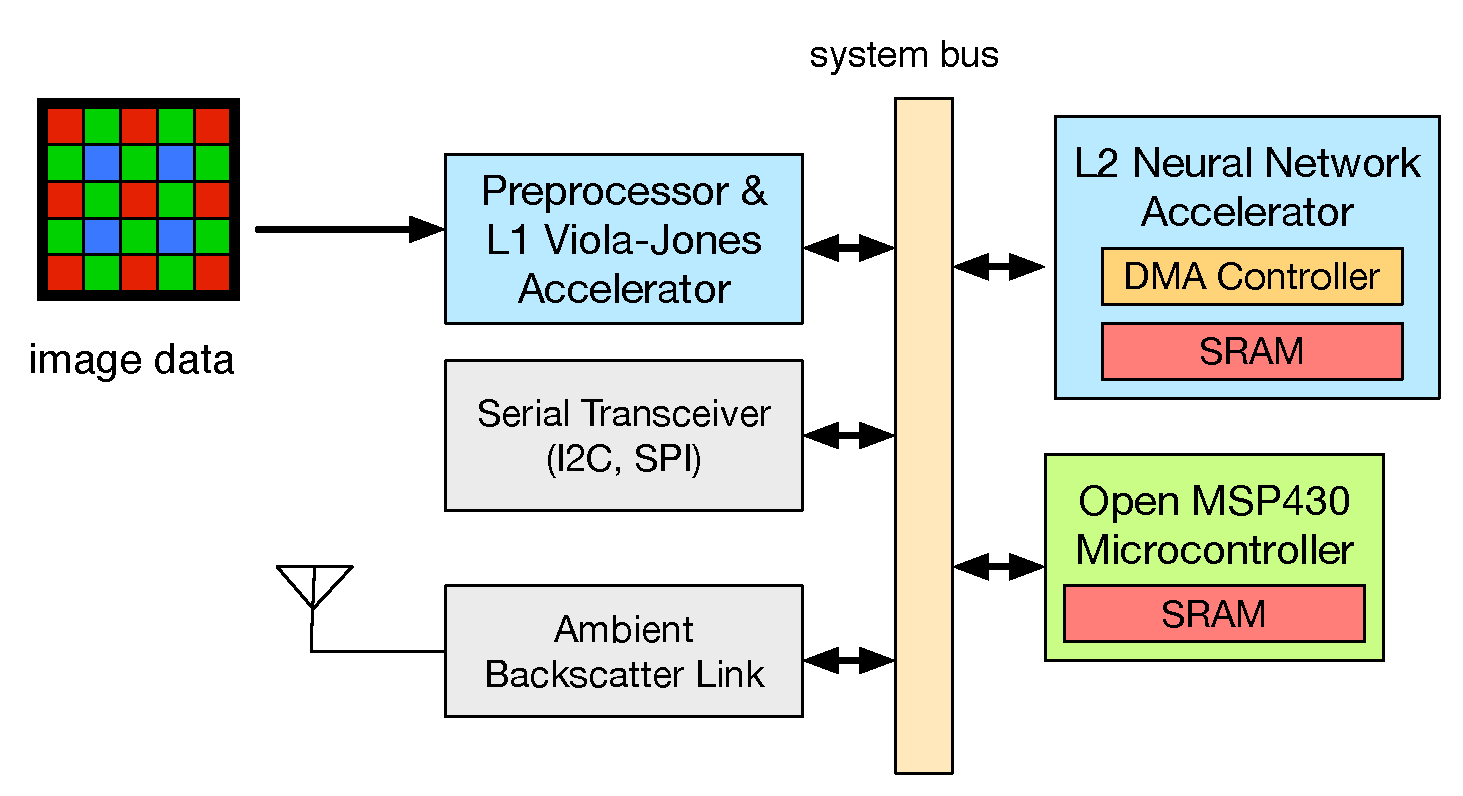
\includegraphics[width=\textwidth]{nsp-figs/system_overview.pdf}
  \caption{OpenMSP-based system overview. }
  \label{fig:OMSP}
\end{marginfigure}


The WISP5.0 is based on the MSP430FR5969 microcontroller with a low-power 3D ADXL362 accelerometer. The WISPCam extends it with a OV7670 camera module that can capture a 176$\times$144 pixel gray scale image and store it in memory with a ~10mJ energy budget.

We envision the described face detection accelerator to be coupled with a neural network accelerator and microcontroller and embedded in a single chip, where the image sensors and processors are fabricated on the same die. This allows low-cost access to the sensor data, since the cost of data movement is significantly reduced. One can use low-power circuits to perform motion detection. This means that a frame is captured only when motion happens, yielding a significant energy reduction. The motion detection circuit in \cite{multipower-isscc13} can be seen as a Level-0 (L0) accelerator that filters the frames, before sending them to the L1 accelerator for face detection.

\subsection{Neural network face authentication}

\begin{marginfigure}
  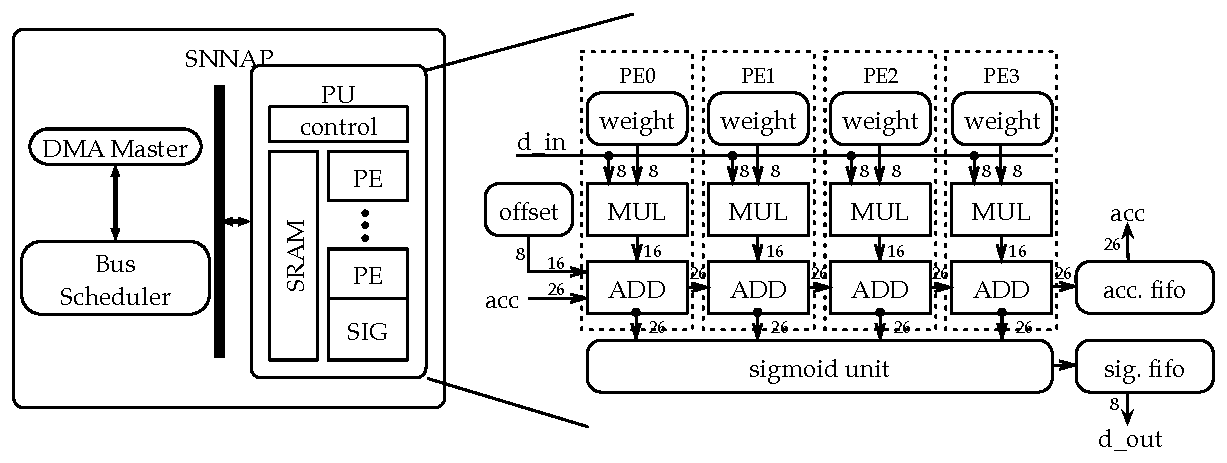
\includegraphics[width=\textwidth]{nsp-figs/snnap_pu_new.pdf}
  \caption{NN microarchitecture and processing element details.}
  \label{fig:snnap-pu}
\end{marginfigure}

NNs are considered state-of-the-art for image inference~\cite{amos2016openface}, so for our face authentication task, we employ a systolic NN design, based on SNNAP~\cite{snnap,moreau-bitwidth}.
We train the NNs with Fast Artificial Neural Network Library (FANN)~\cite{fann}, a popular open-sourced NN library.
Our NN microarchitecture uses a single processing unit with multiple processing elements.
We found that,because our face authentication pipeline has wide layers, this design configuration presented enough data parallelism to keep functional unit utilization high for a single processing unit.
Figure~\ref{fig:snnap-pu} shows the datapath of a processing unit composed of four 8-bit processing elements (PEs).

\section{In-camera face detection using Viola-Jones face detection}

\subsection{VJ algorithm tradeoffs.}
We first tune the parameters of the VJ algorithm in search of the optimal point in the energy-accuracy tradeoff space.
Recall that the Viola-Jones algorithm scans a fixed-size window across an image,
evaluating a classifier at each x-y location, and then scales the window and repeats
the search for larger-sized faces.
A high-level description of this algorithm is listed in Figure~\ref{fig:vj-algo}.

\begin{marginfigure}
\begin{tabular}{c}  % the tabular makes the listing as small as possible and centers it
\begin{lstlisting}
for x in range(0,image_width):
  for y in range(0,image_height):
    faces += classifier_kernel(x, y, window)
    window = window * scale_factor
    if window > max(image_width, image_height):
      exit()
\end{lstlisting}
\end{tabular}
\caption{Nested loops of classifier invocations for VJ.}
\label{fig:vj-algo}
\end{marginfigure}


VJ classifiers are structured to minimize computation in non-face windows: executing a full positive face detection incurs a larger computation cost, whereas deciding early that there is no face has a much lower cost.
The parameters of \textit{window scale factor}, the size of the window scanned looking for a face, and \textit{window step size}, the space between windows evaluated over the image, affect the number of kernel invocations, as shown in Figure~\ref{fig:vj-algo}.

\paragraph{Window scale factor.}
To find faces of
multiple sizes, the window (and features evaluated) are scaled by a scaling factor. This scaling factor
affects the number of iterations over an image the classifier must perform, and thus can greatly impact
energy cost. Viola and Jones use a scale factor of 1.25 in their original evaluation, while the OpenCV
implementation uses a scale factor of 1.1. For our implementation, we considered scale factors between 1.05
and 2 and explored how they impacted accuracy on a fixed-size image.

\begin{figure*}
\noindent
      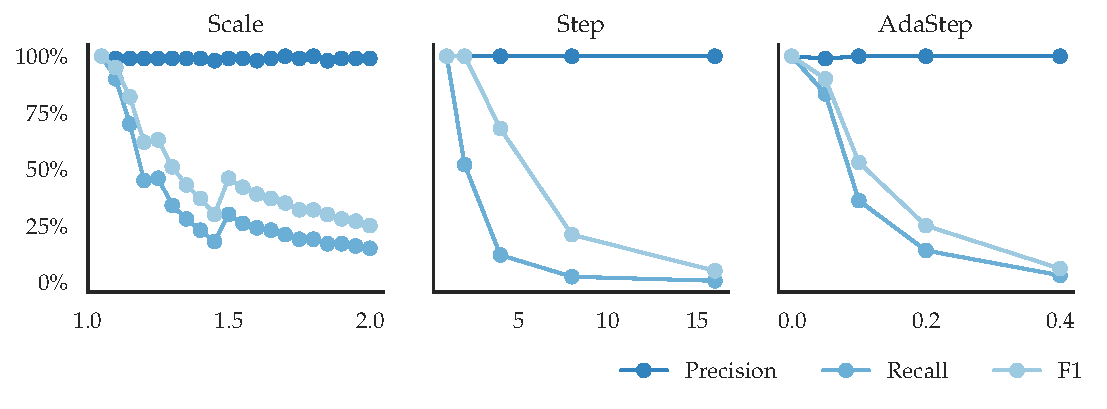
\includegraphics[width=.8\textwidth,right]{nsp-figs/vj_algo_accuracy2.pdf}
    \caption{Impact of VJ parameters on relative accuracy.}
    \label{fig:vj-accuracy}

\end{figure*}

As shown in Figure~\ref{fig:vj-accuracy}, increasing the window scaling factor impacts recall but not precision,
because the number of missed faces grows while maintaining a low false positive rate. In this experiment, accuracy is normalized to the smallest window scale factor, 1.05.

\paragraph{Pixel step number.}
The rectangular features in a cascade classifier are averages over pixel intensities,
and are thus insensitive to small changes in translation and scale. Consequently,
an implementation of the algorithm can safely skip positions in both the x and y direction while
maintaining accuracy. This is especially true in larger window scales, where shifting the window
by a few pixels does not largely impact the results for a single feature.
To demonstrate, we explore the impact of pixel step size on accuracy in Figure~\ref{fig:vj-accuracy}, normalizing
accuracy to a 1-pixel step size.  We find that increasing the window step number has little
impact on precision, but dramatically reduces recall.

We also evaluate stepping the window
position adaptively, as a small percentage of the window size. For the smallest $20\times 20$-pixel window, we use a
pixel step number of 1, 5\% of the window size. The step size of the window grows linearly as a
percentage of the window size. Figure~\ref{fig:vj-accuracy} shows that adaptive stepping the window as a percentage of the window size retains
higher recall than a constant step size. Accuracy here is normalized to the step percentage
of 2.5\%.
This parameter selection results in 86\% less invocations of the VJ classifier and no loss in accuracy for our real-world workloads.

\subsection{Classifier structure}
The structure of the classifier, or the number of stages and features in each stage,
impacts the energy efficiency of the architecture as well as the accuracy of the
classifier. Prior work in hardware implementation of Viola-Jones has used
classifiers ranging from 5 stages with 5 features per stage to 30 stages and
hundreds of features per stage. We trained cascade classifiers at a range of
configuration points with OpenCV and face images from
the AT\&T Database of Faces \cite{attfaces}, and evaluated their impact on accuracy, storage, and
frame rate. The results are compiled in Table~\ref{table:vj-clsfr-sizes}.

\begin{table}[h]
  \centering
\begin{tabular}{cccccc}
\hline
Stages  & Features/Stage  & Precision & Recall & Storage (KB)  \\ \hline
5       &       5         & 0.155     & 0.146  & 1.797         \\
5     &         50        & 0.047     & 0.796  & 6.578        \\
15    &         10       & 0.043     & 0.641  & 10.102     \\
10    &         33       & 0.099     & 0.913  & 17.445     \\
15    &         50       & 0.326     & 0.854  & 33.867         \\
20    &         50       & 0.52      & 0.757  & 50.781      \\
22    &         500      & 0.638     & 0.806  & 58.812     \\
30    &         50       & 0.731     & 0.66   & 80.32      \\
\hline
\end{tabular}

\caption{Accuracy and storage for Viola-Jones classifiers.}
\label{table:vj-clsfr-sizes}
\end{table}



\paragraph{Accuracy.}
Smaller classifiers are cheaper but lead to reduced accuracy
for the overall system.
Deploying a small classifier configuration such as Classifier $5\times 5$ seems reasonable
because of its small storage size, but its low
precision and recall deliver less gains than using no accelerator at all. Increasing
the number of stages and features improves the classifier's overall accuracy, resulting
in better system efficiency. In Table~\ref{table:vj-clsfr-sizes},
Classifier $10\times 33$ has the best recall, but its precision
is low, and its execution would not filter out many false positives. Classifier
$20\times 50$, however, reduces the false positive rate by 50\% with only a 15\% loss in precision.

\begin{marginfigure}
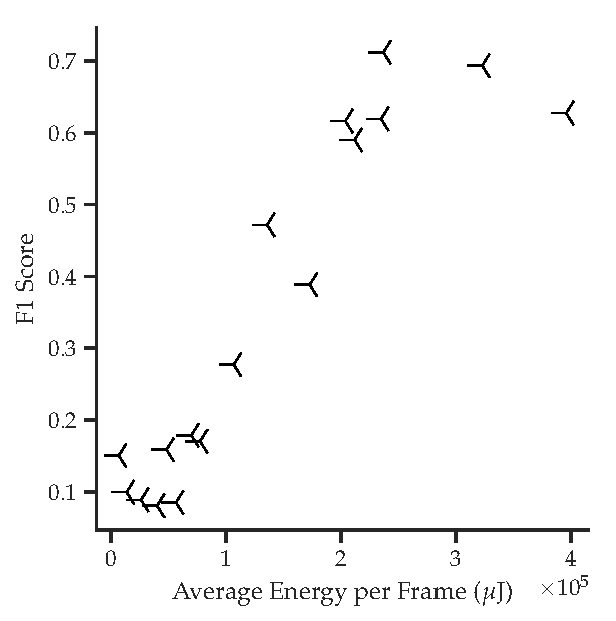
\includegraphics[width=\textwidth]{nsp-figs/eval_vj_energ_acc2.pdf}
    \caption{VJ energy-accuracy trade-off.}
    \label{fig:vj-tradeoff}
\end{marginfigure}

\paragraph{Energy-accuracy Trade-off.} The average energy expended to evaluate an image window
is a function of both the hardware design and the accuracy of the classifier being evaluated.
Small classifiers that have very few features per stage, like Classifier 5$\times$5 from
Table~\ref{table:vj-clsfr-sizes}, have very low recall rates. Low recall rates means they detect less
faces, and, consequently, these classifiers display low energy consumption. Improving recall by
adding more features to a classifier results in more energy-hungry classifier execution. As recall
improves, however, it becomes difficult to maintain high precision. Classifiers with lower precision,
which classify more false positives, will spend more energy overall than those with higher precision.
This effect is demonstrated in Figure~\ref{fig:vj-tradeoff}.


\subsection{VJ streaming microarchitecture.}
Many VJ accelerators exist in the literature for different application domains and power envelopes.
The key observation that facilitates sub-mW power consumption for our accelerator is to process the data in a streaming fashion, leveraging the nature of the pixel stream.
Designing an accelerator in the camera node allows us to process the data in the flow of the input pixel stream, rather than repeatedly fetching blocks from a memory.
By co-designing the accelerator to work with the established dataflow, we reduce storage costs, reducing power consumption.
This also allows us to reduce latency in delivering results to the next step in the pipeline---rather than blocking for a whole frame, the accelerator can deliver partial frame windows with faces as they are processed.

A high-level block diagram of the microarchitecture is shown in Figure~\ref{fig:vj-block}. The accelerator consists of two functional modules: (i) the integral image accumulator, which transforms the image for easy feature extraction, and (ii) the cascade classifier implementation, which evaluates features and computes the classifier result for an image window.

\begin{marginfigure}
      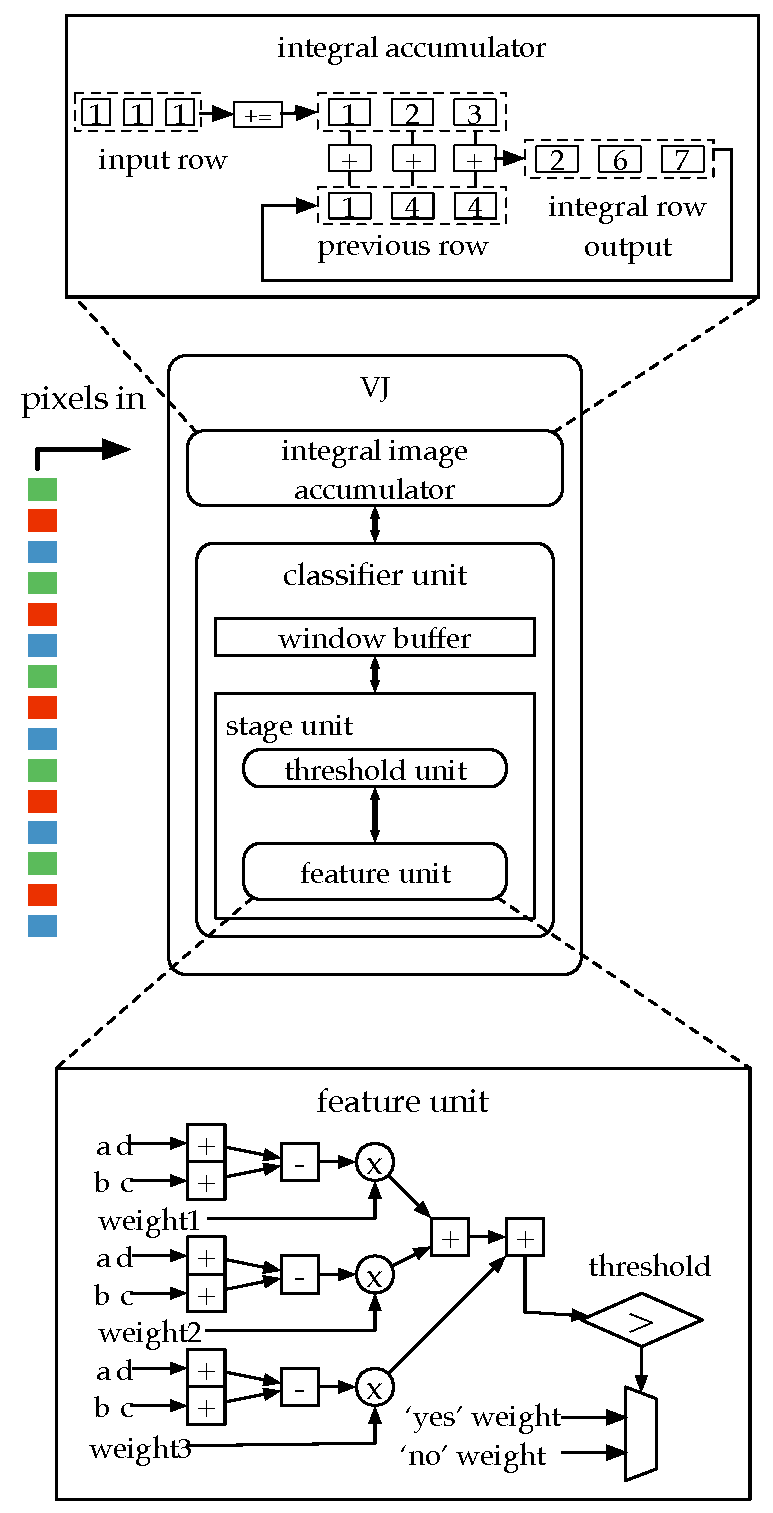
\includegraphics[width=\textwidth]{nsp-figs/vj_arch.pdf}
    \caption{Proposed Viola-Jones accelerator architecture.}

    \label{fig:vj-block}
\end{marginfigure}

%
\paragraph{Integral image processing.} The integral image is computed by summing the pixels above and to the left of
a given pixel. In our design, we
compute the integral image iteratively using two row buffers---one to store the
previous row and one to store the current row. By maintaining
a cumulative row sum in the current row buffer and the previous integral image row
it is possible to compute the integral image with minimal storage.

% \begin{figure}[h]
% \centering
%     \begin{center}
%       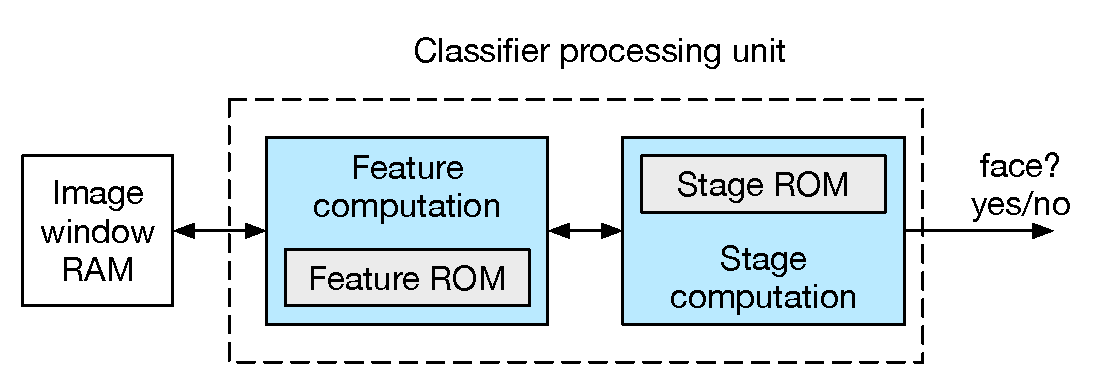
\includegraphics[width=0.5\textwidth]{nsp-figs/cascade_pu.pdf}
%     \end{center}
%     \caption{Cascade classifier processing unit.}
%     \label{fig:cascade-structure}
% \end{figure}

% \paragraph{Cascade classifier computation.} Figure~\ref{fig:cascade-structure} shows a high-level overview of the classifier processing unit. This unit is designed to optimize for minimal energy and area. It implements the logic for computing a single feature and a single stage, and it is
% time-multiplexed to evaluate different features and stage computations. Computation and memory
% accesses are tightly pipelined within the feature and stage units, yielding a fast feature evaluation.


\paragraph{Storage requirements.}
Larger classifiers require more storage for the many feature and stage weights used.
We use small ROMs to store feature and stage weights, and use 65 KB of storage in our design,
split across two units, a 1KB ROM for stage data and a 64 KB for feature computation. This capacity
can accommodate all but one of the classifiers in Table~\ref{table:vj-clsfr-sizes}.

\paragraph{Bit-width reduction} We convert all floating-point computations
to fixed-point to reduce overall energy dissipation. The
data-path for computation on integral image pixels is already large, because 18-bit pixels are
required to store an integral image from 8-bit sensor image. To mitigate the impact of this large data-path,
we reduce the bit-width of feature and stage weights to 16-bit with negligible accuracy loss.

By computing the integral image for a whole image while buffering just two rows, we use significantly less storage than if we had buffered the whole image to compute the integral image result: for our WISPCam workload, we use less than 1kB to hold the necessary rows for integral image output, whereas buffering the whole image would require a 57kB buffer.
We also included a unit to transform face windows from integral image form to standard images before they are transferred to later stages of a camera pipeline.

% Energy efficiency is a central goal of the proposed architecture, and application performance requirements allow the design to run slower than the nominal frequency $f_{max}$ at 0.9V. To absorb the timing slack in the form of energy savings, we aggressively scale the system voltage and derive the optimal voltage for the entire SoC subject to application constraints.

% The theoretical optimal voltage $V^*$ is that which minimizes the system energy $E$, given by

% \begin{equation}
% E_{tot} = E_{dyn} + E_{leak} = \frac{P_{dyn}}{f(V)} + \frac{I_{leak}(V) V}{f(V)}
% \end{equation}

% \noindent where $E_{leak}$ and $E_{dyn}$ are the system leakage and dynamic energies, respectively, and $f(V)$ is the maximum system frequency as a function of voltage \cite{weste_harris}. Since the dominant portion of the leakage energy is attributed to memory \cite{shidiannao}, we can approximate $I_{leak}$ with the leakage attributed to SRAM. For each system module (OpenMSP430, ANN, VJ), we evaluate the dynamic power ($P_{dyn}$) post-synthesis with Synopsys PrimeTime PX.

% For the SRAM leakage term $I_{leak}(V)$, we use the sub-threshold leakage-current relationship \cite{weste_harris} to model the dependence of leakage on voltage. For the frequency function, we construct a system frequency approximation based on previous low-voltage 65nm SRAM implementations \cite{qazi_sram} \cite{verma_sram}.

% \begin{figure}[h]
% \centering
%     \begin{center}
%       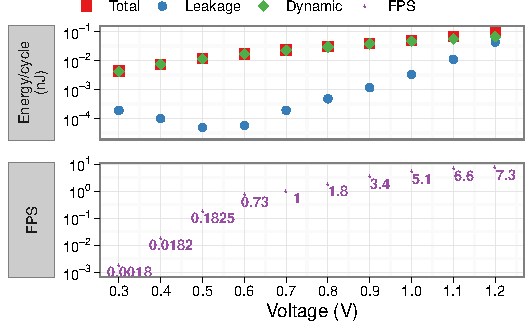
\includegraphics[width=0.5\textwidth]{nsp-figs/vj_voltage.pdf}
%     \end{center}
%     \caption{Energy components}
%     \label{fig:system_voltage}
% \end{figure}

% With the terms described above we derive the dynamic and leakage energy per cycle for a full ANN, VJ, and OpenMSP430 combination. While there is an energy minima at 0.5V for the leakage energy (Figure~\ref{fig:system_voltage}), the dynamic and total energies continue to decrease into the sub-threshold region. Hence, the optimal the system voltage is determined by the minimum voltage at which performance constraints are satisfied. For our application, we select the 0.7V/28 MHz operating point, which satisfies the application performance constraint of 1 FPS.

\section{Experimental results}
Table~\ref{table:fa-hardware} describes the details of our evaluation. We compared the performance and energy of our accelerator configuration against a software baseline running on an MSP430, a low-power microprocessor on the WISPCam. We wrote an NN micro-benchmark trained for face authentication, and emulated execution on a synthesized OpenMSP430 design. We then compared the performance of the NN and face detection (FD) accelerators. To obtain accurate energy estimates, we measure the initiation interval of the hardware pipelines in functional simulation
and use power dissipation numbers derived from PTPX to produce energy estimates.


\begin{table}[h]
  \caption[][-30pt]{Full face authentication system parameters.}
  \label{table:fa-hardware}
 \resizebox{1.5\linewidth}{!}{%
  \centering
    {
\begin{tabular}{llllllll}
\multicolumn{2}{c}{\textbf{Experimental Parameters}} & \multicolumn{2}{c}{\textbf{VJ Accelerator}} & \multicolumn{2}{c}{\textbf{NN Accelerator}} & \multicolumn{2}{c}{\textbf{OpenMSP430~\cite{OpenMSP430}}}  \\ \midrule
Technology & 65nm TSMC GP HVT & Memory & 1kB frame buffer & Memory & 512kB IM, 4kB DM & Memory & 2kB IM, 2kB DM \\
Tool Chain & Synposys & Datapath & 16-bit custom logic & Datapath & 8$\times$8-bit PEs & ALU & 16-bit with multiply \\
C Compiler & TI msp430-gcc~\cite{msp430gcc} & Cascade & 10$\times$33 & Sigmoid & 256B LUT & Power & 181\textmu W \\
SRAM & ARM compiler + derivation & Input & 176$\times$144 pixel stream & Input & 400-pixel image window & Area & 0.12$mm\textsuperscript{2}$ \\
Vdd & Low-voltage, 0.7V & Power & 337\textmu W & Power & 393\textmu W &  &  \\
Freq & 27.9MHz & Area & 0.06$mm\textsuperscript{2}$ & Area & 0.38$mm\textsuperscript{2}$ &  &  \\ \midrule
\end{tabular}

    }
    }

\end{table}

\subsection{Physical implementation and optimization}

We implemented our design in Verilog, synthesized with Synopsys Design Compiler using the TSMC 65nm Gplus Standard VT library, and performed place-and-route with Synopsys IC Compiler. SRAM macros are generated with an ARM Advantage memory compiler. A layout shot of our system components is shown in Figure~\ref{fig:layout_shot}. To find the optimal system voltage, we derive the static and dynamic components of the total system energy and select the minimum-energy voltage that still satisfies system performance requirements.

\begin{marginfigure}
\centering
    \begin{center}
      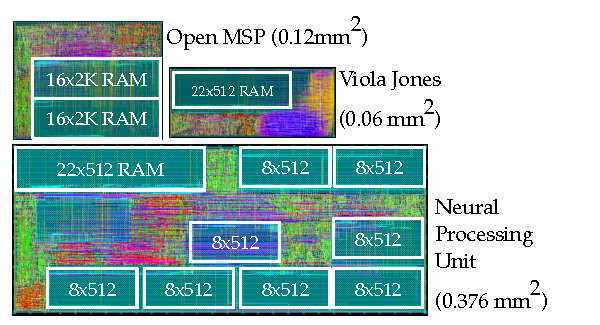
\includegraphics[width=1.2\textwidth]{nsp-figs/layout.pdf}
    \end{center}
    \caption{Layout shot of all three designs}
    \label{fig:layout_shot}
\end{marginfigure}


In our evaluation, system requirements constrain the baseline choice: the MSP430 is the only processor operating within the power constraints of current energy-harvesting systems.
Higher-performance embedded processors, while able to execute our application with better performance than an MSP430, were limited by the power budget required.
In prior NN-accelerator work, the most appropriate comparison is ShiDianNao~\cite{shidiannao}, which also operates at $ \sim$300mW, still significantly higher-power than our design.

\paragraph{Comparing Viola-Jones against neural networks for face detection}
We compared the performance of both Viola-Jones and neural network accelerators
on the same task: face detection. While neural networks offer flexibility,
which make them compelling to solve a myriad of classification problems, but the
specialization of the Viola-Jones accelerator results in better performance and
accuracy.

For the face detection application, the Viola-Jones accelerator presents
a 2.1$\times$ energy improvement compared to running a neural network. On top of that energy reduction, Viola-Jones offers much improved classification performance.
Specifically we found in practice that Viola-Jones had substantially better
false-positive rate than the neural network which has a more approximate nature.
The efficiency benefit of the Viola-Jones classifier
can attributed to its ability to spend little energy on the common case, when a
window contains no faces.

\begin{marginfigure}
\centering
    \begin{center}
      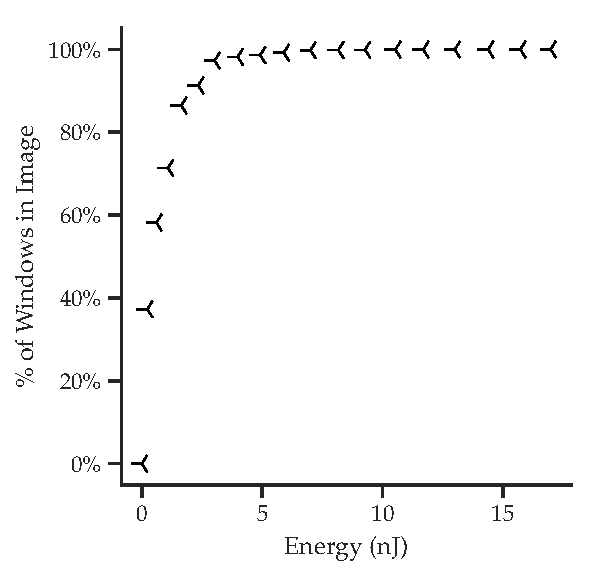
\includegraphics[width=\textwidth]{nsp-figs/eval_vj_cdf2.pdf}
    \end{center}
\caption{VJ energy CDF over all windows in an image.}
\label{fig:vj-cdf}
\end{marginfigure}

Figure~\ref{fig:vj-cdf} shows the
distribution of features across windows in a typical 176$\times$144 image with a single face -- only 0.01\%
of windows need to compute the full classifier.

\subsection{Tradeoffs in computation and communication.} To improve energy efficiency, we evaluate hybrid approaches, which first use VJ-based face-detection
to filter out the windows that do not contain faces, to only feed the small fraction of frames that do contain faces to the neural network that performs face identification.
This approach takes advantage of the efficiency of the Viola-Jones accelerator, to reduce the cost of performing face identification with a neural network accelerator.


\paragraph{Methodology for evaluating real-world workloads.} To consider the computation and communication power of our accelerators and the CPU baseline, we evaluated all configurations of the face authentication pipeline on experimentally-collected videos of real-world workloads.
The dataset contains video scenarios we crafted to be representative of mobile face authentication in the wild, primarily surveillance-style security videos of a lab and a videos from a wearable-style device with an always-on camera.
We collected seven videos in total, each 60-75 seconds in length: three for the security monitoring workload and four for the wearable-in-action workloads.
To match the system design requirements of an energy-harvesting platform, we captured and processed the video at 1 FPS.

Using these benchmarks and the power/performance characteristics of our accelerators, we derived the input bandwidth and resulting power consumption for each computational block in every configuration of the system. To derive the cost to offload image data, we used previously reported communication power numbers~\cite{wispcam}.

\paragraph{Computation-communication tradeoffs in real-world workloads.} Figure~\ref{fig:all-face-auth-configs} shows our results for the full system of image sensor capture, motion detection, FD, and NN face authentication, comparing total power consumption on combinations of the ASIC designs described in this section. Because the CPU could not compute the face recognition kernel on even one 400-pixel window at 1 FPS, we did not consider the results in this section. The configurations including CPU face authentication consume 2-5 orders of magnitude more power overall than the full-ASIC design we implemented.


\begin{figure*}[h]
\centering
    \begin{center}
      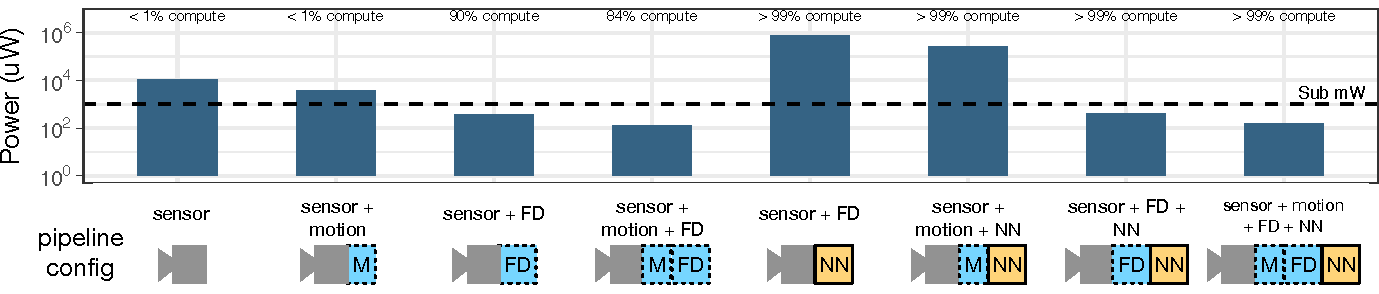
\includegraphics[width=1.0\textwidth]{nsp-figs/FA_compute_comp_v5.pdf}
    \end{center}
    \caption{The total power for different ASIC accelerator configurations is typically dominated by either computation or communication power. The lowest-power solution uses the motion and face detection filters and offloads the NN. }
    \label{fig:all-face-auth-configs}
\end{figure*}

Figure~\ref{fig:full-face-auth-pipeline} shows the detailed power breakdown between computation and communication for the full system in silicon. The computation power is the sum of power at that block and the processing blocks preceding it, and the communication power is the cost to transfer the output of that block. As expected, the computation power increases as more blocks process the data while the communication power decreases, but not at the same rate. Counterintuitively, the total power increases by 28\% after performing the NN, indicating that \textit{it is more power-efficient to offload after motion and face detection, rather than performing the full pipeline.} Even though the NN only needs to communicate a 1-bit response, the cost of computation increases dramatically in comparison to the decrease in communication power. This result indicates that it is more cost-effective to offload the neural network than process it in-camera, in this power-constrained application domain.

\begin{marginfigure}
\centering
    \begin{center}
      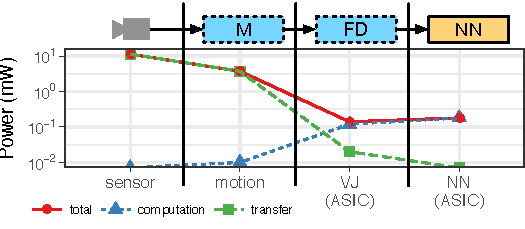
\includegraphics[width=\textwidth]{nsp-figs/FA_compute_compress_4up_fig.pdf}
    \end{center}
    \caption{Computation and communication power after each ASIC block in the ``full pipeline'' configuration.}
    \label{fig:full-face-auth-pipeline}
\end{marginfigure}

So, why not always offload neural networks? We examined the extent to which different constraints in our design contributed to our results. We found that if the communication power cost per pixel grew by 2.68$\times$, it would be more power-efficient to perform the NN in-camera. Our evaluation sourced communication power data from work using a directed RFID reader, and RF-based energy harvesting systems may not always deliver consistent power.

\subsection{Discussion}

Analysis of the video workloads highlights the benefits and limitations of our filtering approach at the application level. Importantly, the complete pipeline, consisting of motion detection, VJ, and NN, did not eliminate any true faces in any of our workloads. Using these filtering steps reduces data bandwidth, but we find that the extent of the data reduction could be improved. Motion detection often is triggered in innocuous situations, such as when people pass by in a frame or a mobile device is carried while walking. Our face detector misclassifies many false positives as faces, and also detects faces in static posters and photos. We examined the results of one of our security authentication workloads to illustrate: out of 62 frames of video, 12 frames were accepted through a motion detection block. In those 12 frames, the VJ detector passed forty 400-pixel face windows to the NN classifier. Visual inspection of those 40 faces found that 10\% were false positives---with a perfect face detector that only detected true faces, the power to offload or compute the NN on-device would be reduced.

To investigate the impact of image size on the tradeoff between in-camera and offloading, we scaled our evaluation from the low-resolution images produced by the WISPCam to high-resolution mobile camera images. We found that keeping the neural network in-camera became power-efficient at 8 megapixels or greater. Finally, while offloading data may be more power-efficient, privacy and bandwidth concerns may lead designers to opt for a more localized solution when processing image data for face authentication tasks. These results indicate that as mobile camera devices become more sophisticated, architectures will have to become increasingly specialized to deliver low-power in-camera results.

%%%%%%%%% bit bucket



%WISPCam data
%Resolution 176*144
%Capturing and storing 8.51 mJ in 115ms
%Transferring 11.34 mJ in 3s
%Passive Infrared (PIR) motion sensor 10uW
% \begin{figure}[ht]
% \centering
%     \begin{center}
%       \includegraphics[width=0.5\textwidth]{./figs/FA_pipeline_base_with_example.pdf}
%     \end{center}
%     \vspace{-1.5em}
%     \caption{Continuous face authentication pipeline. }
%     \label{fig:fa_pipeline_base}
% \end{figure}

% put an explanation of one of the videos and the breakdown of the paper

% \begin{table}[tb]
%   \centering
%   \begin{tabular}{ l @{\hskip 6pt}l @{\hskip 6pt}l @{\hskip 6pt}l  }
% \toprule
% \textbf{Platform} & \textbf{Configuration} & \textbf{FPS} & \textbf{Output (pixels)} \\
% \midrule
% % Base & & & \\
% Base & Sensor & & 25344\\
% & Sensor + Motion & & 25344\\
% \midrule
% % ASIC & & & \\
% ASIC & Sensor + VJ & & 400\\
% & Sensor + Motion + VJ & & 400\\
% & Sensor + NN & & 1\\
% & Sensor + Motion + NN & & 1\\
% & Sensor + VJ + NN & & 1\\
% & Sensor + VJ + NN & & 1\\
% \midrule
% % CPU & & & \\
% CPU & Sensor + VJ & & 400\\
% & Sensor + Motion + VJ & & 400\\
% & Sensor + NN & & 1\\
% & Sensor + Motion + NN &  & 1\\
% & Sensor + VJ + NN &  & 1\\
% & Sensor + VJ + NN &  & 1\\
% \bottomrule
% \label{tab:recog_fps_bw}
% \end{tabular}


% \caption{Processing speed and output bandwidth for different configurations of accelerators on ASIC and an MSP430 CPU. }
% \label{table:fa-fps-communication-bandwidth}
% \end{table}


% Using our model, the resulting pipeline is \todo{[final model here]}. Our near-sensor design space
% exploration finds that a standalone CNN accelerator can achieve significant gains in performance and
% efficiency when coupled with a low-power face detection accelerator, but does not ever make sense to be done in camera. We evaluated on real world situations~\todo{explain in more detail}. Figure~\ref{fig:face_recog_configs} shows all the potential configurations and their resulting power consumption.

% There are two scnearios in which it could make sense: 1) if the cost of communication is higher and 2) if we relax accuracy/bitwidth/etc. Also, privacy.
